\documentclass[border=2pt]{standalone}
\usepackage{tikz}
\usetikzlibrary{arrows.meta,positioning,shapes.arrows}
\begin{document}
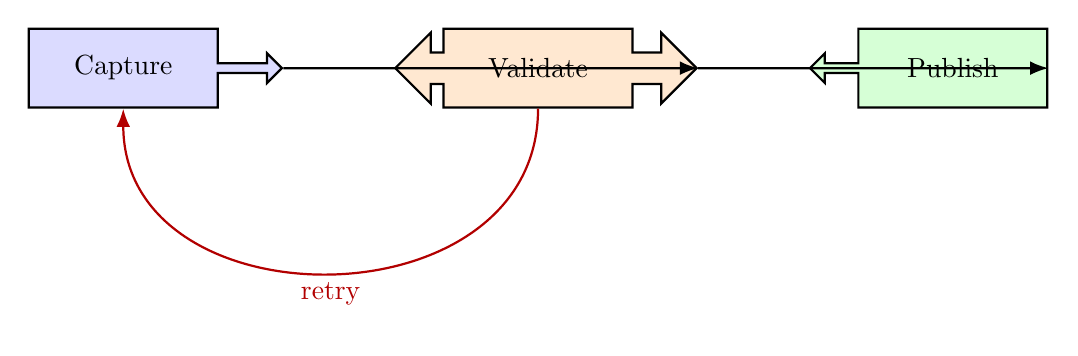
\begin{tikzpicture}[
  >=Latex,
  node distance=14mm,
  every node/.style={draw,arrow box,minimum width=24mm,minimum height=10mm,align=center},
  every path/.style={thick}
]
  \node[fill=blue!14,arrow box arrows={east:8mm}] (capture) {Capture};
  \node[right=of capture,fill=orange!18,
    arrow box arrows={west:6mm,east:8mm},
    arrow box shaft width=4mm,arrow box head extend=2.5mm] (validate) {Validate};
  \node[right=of validate,fill=green!16,
    arrow box arrows={west:6mm}] (publish) {Publish};
  \draw[->] (capture) -- (validate);
  \draw[->] (validate) -- (publish);
  \draw[->,red!70!black] (validate.south) to[out=-90,in=-90,looseness=1.35]
    node[below,draw=none,shape=rectangle,minimum width=0pt,minimum height=0pt]{retry} (capture.south);
\end{tikzpicture}
\end{document}
